\documentclass[a4paper,11pt]{article}
\usepackage[utf8]{inputenc}
\usepackage[spanish]{babel}
\usepackage[left=2cm, right=2cm, top=2cm, bottom=2cm]{geometry}
\usepackage{graphicx}
\usepackage{here}
\newcommand{\mbf}{\mathbf} 
\newcommand{\mrm}{\mathrm}
\usepackage{amsmath, amsthm, amssymb, amsfonts}
\title{Segunda práctica calificada: MC585A}
\author{Josue Huaroto Villavicencio\\
Código: 20174070I}
\begin{document}
\maketitle
\section*{Problema 1. Se adjunta la imagen de un soporte soldado con dos cordones horizontales y 2 verticales. Soportarán una carga vertical de 7000$\,$lb. Hallar el tamaño del cordón filete. Las especificaciones son:}
\textbf{Cordón de filete: E60-XX. $\mbf{S_{w}} =$ 12700 PSI, $\mbf{S_{s} =}$ 15000 PSI.}
\begin{figure}[H]
    \centering
    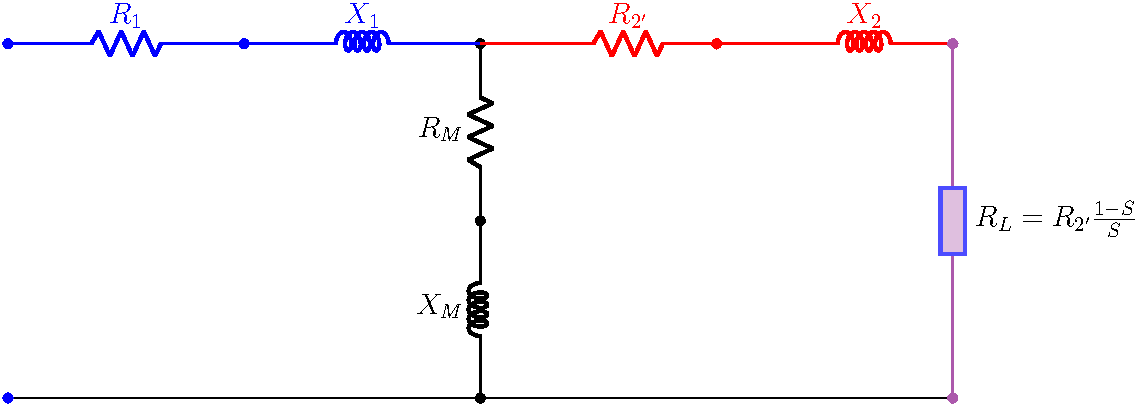
\includegraphics[scale=1.5]{d1.pdf}
\end{figure}
\subsection*{Pregunta 1.1. Hacer el análisis y los efectos de la carga vertical de 7000$\,$lb en los puntos externos 1, 2, 3, 4. El sistema de coordenadas está indicado en la figura para ubicar con precisión las fuerzas sobre los puntos.}
\begin{figure}[H]
    \centering
    \includegraphics[scale=1.3]{d2.pdf}
\end{figure}
\subsection*{Pregunta 1.2. Analice identificando los efectos generados por la carga de 7000$\,$lb.}
$$
P = 7000\,\mrm{lb}
$$
\begin{itemize}
    \item Carga de corte directo: $f^{(1)}$ (-y)
    \item Carga de corte por momento flector: $f^{(2)}_{3H} = f^{(2)}_{4H}$ (-x)
    \item Carga de corte por torque: $f^{(3)}_{1H}$ (+x)
\end{itemize}
\subsection*{Pregunta 2.0. Hallar el centro de gravedad de los cordones.}
$$
\bar{y} = \frac{d^{2}}{2(b+d)} = \frac{8^{2}}{2(8+8)} = \frac{64}{32} = 2
$$
\textbf{Módulos de los cordones:\\}
\begin{itemize}
    \item $z_{xi}$: Módulo de los cordones verticales en punto inferior.
    \item $z_{xs}$: Módulo de los cordones horizontales en punto superior.
\end{itemize}
\begin{align*}
    z_{3i} = z_{4i} &= \frac{4bd^{2}+d^{3}}{6b+3d} = \frac{4\times 8\times 8^{2} + 8^{3}}{6(8) + 3(8)} = 35.555\\
    z_{1s} = z_{2s} &= \frac{4bd + d^{2}}{3} = 106.666
\end{align*}
\subsection*{Pregunta 3.0. Hallar las fuerzas por los efectos de la carga $P$ de 7000$\,$lb}
\subsection*{Pregunta 3.1. Fuerza de corte directo.}
\begin{align*}
L_{4} &= d - 5/8 = 7.375\,\mrm{pulg}\\
f^{(1)} &= \frac{P}{L_{w}} = \frac{7000}{2(8-\frac{5}{8}) + 8 + (8-0.5)} = 231.40496\,\mrm{lb/pulg}\;(-\mrm{y})
\end{align*}
\subsection*{Pregunta 3.2. Fuerza por momento flector en punto 4 inferior, en punto 2 superior.}
\begin{align*}
M\cdot x &= 5000\cdot 12 = 60000\,\mrm{lb-pulg}\\
f^{(2)}_{4H} &= \frac{M\cdot x}{z_{x} = z_{4i}} = \frac{84000}{35.555} = 2362.5\,\mrm{lb/pulg}\\
f^{(2)}_{1H} &= \frac{M\cdot x}{z_{x} = z_{2s}} = \frac{84000}{106.6666} = 787.5\,\mrm{lb/pulg}\\
f^{(2)}_{2H} &= f^{(2)}_{1H} = 787.5\,\mrm{lb/pulg}
\end{align*}
\subsection*{Pregunta 3.3. Fuerza por torque.}
$$
J_{w} = \frac{d^{3}(4b+d)}{6(b+d)} + \frac{b^{3}}{6} = 298.666\,\mrm{pulg}^{3}
$$
\begin{align*}
    f^{(3)}_{4V} &= \frac{M\cdot x \cdot CH_{4}}{J_{w}} = \frac{21000\times 0.25}{298.6666} = 17.578125\,\mrm{lg/pulg}\;(-\mrm{y})\\
    f^{(3)}_{4H} &= \frac{M\cdot x \cdot CV_{4}}{J_{w}} = \frac{21000\times 6}{298.6666} = 421.875\,\mrm{lg/pulg}\;(-\mrm{x})
\end{align*}
\begin{figure}[H]
    \centering
    \includegraphics[scale=0.7]{d3.png}
\end{figure}
\subsection*{Pregunta 4.0. Calcule las fuerzas resultantes en los puntos 4 y 2.}
\begin{figure}
    \centering
    \includegraphics[scale=1.2]{dib1.pdf}
\end{figure}
\begin{align*}
    f_{RF} &= \sqrt{2362.5^{2} + (17.578125+231.40496)^{2}} = 2375.58389\,\mrm{lb/pulg}\\
    f_{R4} &= 2412.7530627\,\mrm{lb/pulg} 
\end{align*}
\subsection*{Pregunta 5.0. Hallar el tamaño del cordón.}
$$
w = \frac{f_{R4}}{S_{w}} = \frac{2412.7530627\,\mrm{lb/pulg}}{12700\,\mrm{lb/pulg^{2}}} = 0.18998\,\mrm{pulg} \longrightarrow w = \frac{3}{16} = 0.1875''
$$
Según tabla 4.2; el espesor más grueso = 5/8. Considerando cordón E-60XX:
$$
w = \frac{1}{4}\,\mrm{pulg}
$$
\subsection*{Problema 2.}
\subsubsection*{Problema 2.1. Explicar cuáles son los factores que influyen en el cálculo por torque sobre la soldadura.}
\begin{itemize}
    \item Momento polar de inercia ($J_{m}$).
    \item Par de torsión.
    \item Electrodo.
\end{itemize}
\subsubsection*{Problema 2.2. Explicar cuáles son los factores que influyen en el cálculo por flexión sobre la soldadura.}
\begin{itemize}
    \item Momento de Inercia.
    \item Longitud de la soldadura.
    \item Esfuerzo de fluencia.
    \item Electrodo.
\end{itemize}
\end{document}
